\documentclass[a4paper, twocolumn]{article}
\newcommand{\papertitle}{Whitepaper: Community Development of Next Generation Storage and Compute Interfaces for Smart Workflow Processing}

\usepackage[a4paper, margin=2cm]{geometry}

\usepackage[utf8]{inputenc}
\usepackage[T1]{fontenc}
\usepackage{graphicx}
\usepackage[english]{babel}
\usepackage[colorlinks=true,urlcolor=red]{hyperref}
\usepackage{url}
\usepackage{cleveref}
\usepackage{todonotes}

\usepackage{multicol}
\setlength{\columnsep}{1cm}

\usepackage{fancyhdr}
\fancyhead{}
\fancyfoot{}
\fancyhead[l]{\papertitle}
\fancyhead[r]{
\includegraphics[height=1em]{ngi-logo}}
\fancyfoot[r]{\thepage}
\pagestyle{fancy}
\renewcommand{\headrulewidth}{1pt}
\renewcommand{\footrulewidth}{1pt}

\usepackage{titling}
\pretitle{\begin{center}\Large\bfseries}
\posttitle{\end{center}\vskip 0.5em}

\graphicspath{{./assets/}}

\title{\papertitle}

\author{Julian M. Kunkel 
  \textit{University of Reading}
	\and
  Chris Hoffman
  \textit{National Center for Atmospheric Research}
  \and
  B
  \and
  C
}
\date{\today}


\begin{document}
\maketitle
\thispagestyle{fancy}

\section*{Abstract}

The efficient, convenient, and robust execution of data-driven workflows and enhanced data management are key for productivity in scientific computing and computer-aided RD\&E.
Big data tools integrate compute and storage capabilities into a holistic solution demonstrating the benefit of tight integrating while the HPC community still optimizes the compute and storage components independently from each other, and, moreover, independently from the needs of end-to-end user workflows  that ultimately lead to insight.
Even within a single data center, utilizing a homogeneous storage and compute infrastructure efficiently is complex for experts and needs a manual definition.
The efficient management of data and compute capabilities in a heterogeneous environment, however, is an unresolved question as tthe execution of individual tasks from workflows may benefit from alternative hardware architectures and infrastructures.

In this white paper, we describe the vision for the Next-Generation Interface (NGI) initiative that aims to tackle the aforementioned storage and compute challenges in a holistic approach.
Within the NGI consortium, we fuse state-of-the-art concepts into a revolutionary interface by rethinking how data-driven I/O should be done.
From the user perspective, NGI aims to provide an abstraction to data-driven processing and data management.
The NGI interface ultimately will increase the opportunity of implementations for smarter scheduling of compute and storage in heterogeneous environments considering characteristics of workflows and data.
From the system perspective, the vision of NGI aims to derive an execution plan that utilizes the available hardware and software infrastructure within and across data centers but also on small-scale systems.

\section{Introduction}

High-Performance Computing harnesses the fastest hardware components to enable
the execution of tightly coupled applications from science and industry.
Typical use-cases cover the numerical simulation of physical systems or the analysis of large-scale observational data.
While the hardware of HPC systems is on the bleeding edge, the software landscape of the infrastructure is lacking behind modern concepts found in domains like cloud computing.
There are various reasons for the lack of innovation, e.g., the market capitalization is limited; many HPC applications have a life time of a decade; the goal in HPC is to get science done and not to have modern and user-friendly systems.
Therefore, software developed to target the HPC market is rarely used outside data centers; while there is no reason to use developed applications outside this scope, software to aid developers or for managing HPC infrastructure suffers the same cause.
Nowadays, HPC adapts infrastructure software from the enterprise and cloud market as much as possible; at best, adapting (stretching) already existing software packages to the needs of HPC.

From the perspective of big data and cloud solutions, the state-of-the-art in the HPC software ecosystem is perceived as conservative and outdated at least; for example, HPC still uses batch processing and dedicates nodes to the execution of individual applications which were the first concepts implemented at the dawn of computing.
Similar to writing code in assembler, often it is argued that HPC treats user-friendliness and manageability to obtain the best possible performance.
However, as the complexity of systems increases and various alternative storage and compute technologies provide unique characteristics, it is barely possible to define optimal data-driven workflows using low-level constructs for the following reasons:

\begin{itemize}
  \item Compute focus: HPC considers compute, storage, and network as separate resources and focuses on the compute aspects, e.g., I/O requires to retrieve/store data from a compute node.
  While this provides a wonderful separation of concerns, it disregards the opportunity to process data closer to storage or between applications.
  \item Complexity: a data-driven workflow is highly complex and may benefit from using a heterogeneous set of compute and storage technology at the same time.
  Knowing the capabilities, interfaces, and performance characteristics of individual components is mandatory to make best use of them.
  \item Portability: moving from one infrastructure to another or even when modifying the infrastructure requires to rethink and manually adapt the workflow as the characteristics of the overall environment changes.
  \item Cost-efficiency: it is time consuming to utilize low-level constructs often only increasing performance slightly; also, the cost of labor must be taken into account.
  From the perspective of scientists and engineers, the time-to-solution from experimental design to insight matters and not the cost-savings for the public data center.
  \item Conservative users: users are reluctant to change their workflows for the reasons that older workflows are proven to be correct and it is labor intensive to manually adapt workflows.
\end{itemize}

For these reasons, workflows are typically encoded manually and run suboptimally on HPC systems.
Additionally, users of public data center services supply limited information about their experiments, typically the level of detail is like "I need X CPU hours and Y storage capacity" and they have not to proof their ability to use these systems efficiently.
Still, the systems these workflows run on cost up to 100 million of dollars.
Compare this to experiments conducted in physics like the Large Hadron Collider (LHC) at CERN or the Square Kilometer Array (SKA); execution of complex experiments may need years of planning involving the scientists.
While it is important to keep some freedom to conduct ad-hoc experiments, we raise the question what could be achieved by systems and operators knowing workflows in more detail.
We argue that knowledge about workflow execution and overall experimental design helps to
optimize execution of workflows and additionally increase the performance, throughput and  cost-efficiency of the environments, therewith, providing an incentive to users and data-centers that cannot be neglected.

\medskip

With the Next Generation Interfaces initiative, we aim to define a high-level interfaces that, firstly, meets the needs of users and data centers, and, secondly, that allows implementations to exploit the capabilities of current and future storage and compute landscapes.
The remainder of this article is structured as follows: \\
\todo[inline]{TODO}

In \Cref{sec:background}, we provide relevant background information for workflows.
\Cref{sec:challenges}
\Cref{sec:ngiVision}
\Cref{sec:ngWorkflows}
\Cref{sec:community}
\Cref{sec:conclusions}


\section{Workflows}
\label{sec:background}
This section provides an introduction to workflows that solve computational problems, the mandatory steps to encode and setup tasks and describe data, and the relevance of  heterogeneous infrastructure to run workflows.
We focus on high-level considerations that illustrate mandatory concepts.

%Kubernetes

\subsection{Workflow Description}

To solve a computational problem, we can consider to describe the necessary steps from the start to the insight as a workflow.
Such a workflow description must comprise of the individual data processing steps, the expected  products, together with dependencies between the steps and to input.
The nodes can be annotated with characteristics of the individual steps;
data can be annotated with metadata describing its content, the expected data life cycle information, e.g., the value of data and how long should it be kept; tasks can be annotated with the information needed to start processing or with performance models that bound the  expectations for resources (time, memory, storage capacity).

An example execution of a workflow is illustrated in \Cref{fig:workflow} as a graph (we have not shown characteristics and annotations).
Arrows indicate dependencies between nodes that represent tasks and data.
In the example, Task\,1 needs two datasets to perform its work, it directly communicates with Task\,2 and produces Product\,1.
Most of the workflow can run automatically except the manual quality control of the products and the final data usage of Product\,3 at the end.
The last step represents the typical uncertainty of data reuse, when this workflow is created it is unclear how Product\,3 will be used further, it is apparent that it will be.
Further workflows that use the data may be created similarly and use the product as input.

Note that a realistic workflow will be much more complex and involves not a single parallel job execution but many to generate a robust answer to the research question.


\begin{figure}[b]
  \centering
  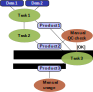
\includegraphics[width=0.75\columnwidth]{workflow}
  \caption{Example High-Level Workflow without Characteristics}
  \label{fig:workflow}
\end{figure}

\subsection{Task Definition}

The high-level interaction of a task with its dependencies is generally specified in the workflow.
A compute task is encoded in a programming language by a developer\footnote{We often treat developer and HPC user as synonyms as a fraction of HPC users are developers for parallel applications to some extent.}.
A team of developers encodes the algorithm that solves the problem -- e.g., in many cases,  scientists that generate a numerical simulation implement the model programmaticially.
Often they use existing libraries that provide a piece of functionality or infrastructure.
In the design phase of the program, a parallel programming paradigm and suitable data structures that allow efficient data processing are chosen.
In the world of parallel computing, the developer must also consider strategies to parallelize the code and data processing; this often involves to use APIs and runtime systems that allow the efficient usage of supercomputers.

While most parts of the algorithm can be a tightly coupled simulation, as part of the algorithm, input data must be fetched and data products are generated which are processes that are executed outside of the main simulation.
Typically, before the input data can be used some kind of preprocessing must be applied, similarly, in the output several known post-processing steps may be applied.
Also, the programmer is responsible for making the optimal decisions on how to map data structures from memory to I/O calls and place these files onto storage systems.

We consider that pre/post-processing are part of the data-driven scope of NGI.
Indeed, we claim the programmer should be able to define the input/output on an abstract fashion and connect processing steps as part of the general workflow.

\subsection{Heterogeneous Infrastructure}

The variety of tasks executed by a single workflow may benefit from a heterogeneous storage and compute infrastructure and potentially even span multiple locations.
\Cref{fig:heterogeneous} shows such an environment but focuses on the computation and storage.
A variety of accelerators (GPU, TPU, FPGAs), active storage, in-memory, and in-network computing technologies provide processing capabilities across and beyond an HPC center optimized for certain workloads.
Data centers typically provide more than one storage and compute class with different characteristics to optimize cost and efficiency.
Likewise, storage is deployed data center wide, locally available to individual nodes, or subsets of nodes (e.g., racks); depending on the need, the characteristics range from predictable low-latency (in-memory storage, NVMe) to online storage (SSD, HDD), to cheap storage for long-term archival (tape).

The processing across geographic locations is nowadays mandatory to tame the data volumes of observational or simulation data.
Also, the lines between cloud computing and HPC are blurry, attempts are made to augment processing by flexibly migrate bursts of computation to cloud environments, ingest data from cloud sources or provided to customers.
Consider a simple scenario where sensor data captured is pre-processed (cleaned) locally, then enriched with an additional data source in a small-scale HPC facility or by using fog computing, then transferred to a data center that performs the number crunching and generates data products.
These data products may be made available on cloud storage to customers for individual processing.

\begin{figure}[b]
  \centering
  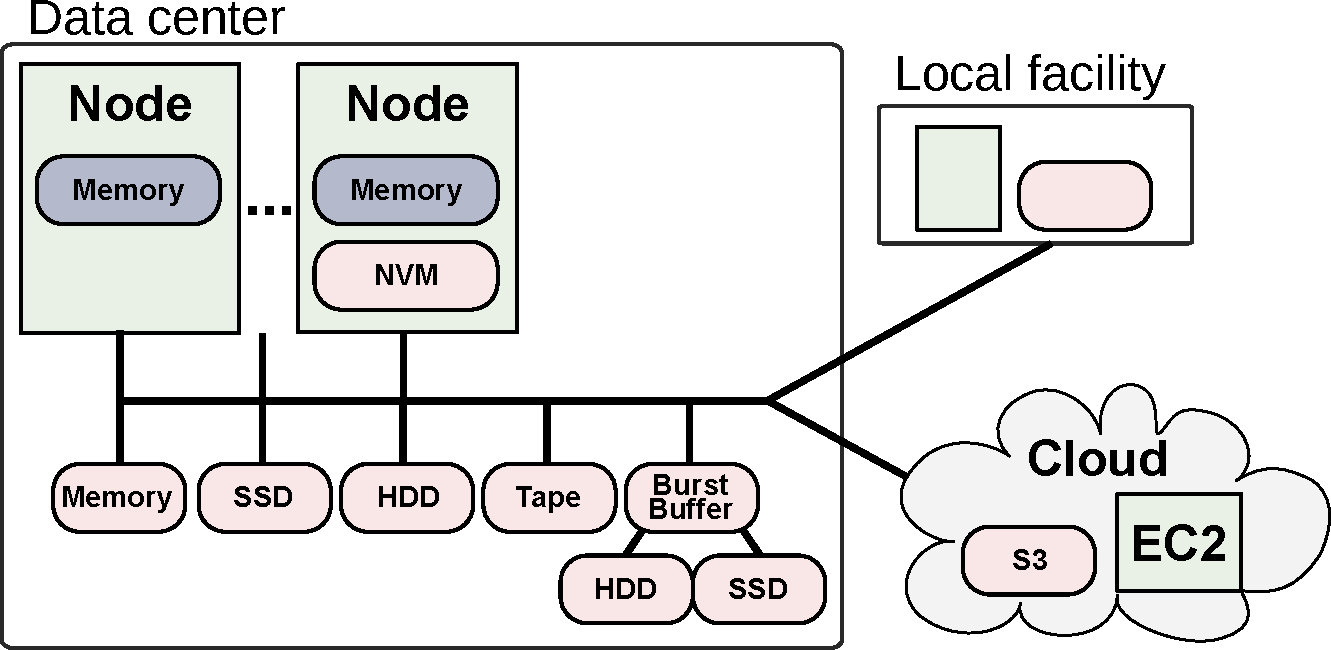
\includegraphics[width=\columnwidth]{system}
  \caption{Example Heterogeneous HPC Landscape}
  \label{fig:heterogeneous}
\end{figure}

\section{Challenges and Limitations}
\label{sec:challenges}
The current HPC environment faces several challenges and limitations in respect to the execution of data-driven workflows.



\paragraph{Low-level interfaces:}
HPC data management and data-flow processing utilizes low-level interfaces.
Storage relies still on traditional file system objects of directories and files -- provided by the POSIX interface or by object storage.
Underlying storage systems are receiving or delivering streams of bytes, and it cannot make any intelligent decisions about how to optimize data layout for performance, or resiliency.
It deals with data blocks and files and requires instructions on how to select and control available optimization strategies.

In practice, applications build up layers so that the application itself is usually working with the data mediated by a library which provides application specific semantics --- but at the lowest level such a library is limited by the underlying storage APIs (POSIX).
This has performance implications due to synchronization in distributed environments but also severely limits the ability of the underlying storage systems to optimize I/O operations.

Data-driven processing suffers similarly, from the high-level view of processes that are executed on a given compute node.


\paragraph{Explicit workflows:}
Typically, as part of shell scripts, users explicitly encode data processing workflows as a sequence of steps consisting of input, compute, and output.
The compute-intense parts (jobs) and their dependencies are managed by a cluster resource manager that dispatches them.
These loosely coupled workflows require that intermediate results are stored on persistent storage to be used by the next task.
Data transfer, however, needs a dominant fraction of energy compared to computation favoring offloading of computation to storage.


\paragraph{Suboptimal Storage Tiering:}
Organizing the data placement on storage tiers is typically performed manually by the developer/user or via policies.
This leads to suboptimal optimizations, is tedious and error prone.

Manual tiering requires the user or application to control the data placement, i.e., storing data (typically in form of files) on a particular storage system and typically moving data between storage by using scripts.
One limitation here is that decisions about how data structures are mapped and packaged into files are made once by the producing application, and cannot be changed without manual intervention by a downstream application.

A policy system (e.g. burst buffer) aims to simplify the data movement for the user but  typically migrates objects in the coarse granularity of files.
However, the semantical information that can be used by a policy system to make decisions is limited, e.g.,  data location, file extension, age of the file.

Any hard-coded decision has significant implications for performance of both applications and systems because the optimal choices about file size and content may be very different for the data production and any subsequent data analysis phase.
In any case, data migration needs resources on the source and the target storage system to copy data.
Thus, it is preferable to direct data to locations where it can be stored and directly used by subsequent workflows; at best coupling the data source producing data with a data consumer to prevent storing intermediate products on persistent storage.

\paragraph{Task and data equality:}

All tasks and data products are handled identically by an HPC system meaning there is no differentiation between individual jobs and data products.
This is problematic as different use cases may not only differ in priority and deadline but as the speed they proceed depends on the critical path of the execution.

Fair enough, batch systems understand a priority for jobs.
However, once a set of nodes is allocated explicitly to a compute job, the job is run exclusively and may utilize shared resources such as storage systems and network as any other job. %-- quality of service features available in hardware are rarely used

This is more sever for data products: a storage system provides a single level of performance and resilience and performance for all use cases.
Theoretically, different fault-tolerance and performance policies can be realized with different storage systems and using management policies.
However, these policies would be coarse-grained and would not account for the priority of the workflow and most importantly the value of data;
the value of data depends on aspects like costs to reproduce the data (can it be re-produced easily), the type of the experiment (test run, production run) and runtime constraints for the overall and potential crucial workflow.
While value and priority should influence fault-tolerance strategies and imply quality of service for performance and availability, in practice this is not the case as the storage just sees blocks and files.

\paragraph{Manual optimization:}
Utilizing the compute and storage characteristics of a heterogeneous environment as depicted in \Cref{fig:heterogeneous} is challenging at least.
The optimization of a single parallel job already is quite challenging.
To make optimal use of available features, programmers and users are forced to think about technological aspects and terms, e.g., setting low-level MPI hints for file striping, while they understand their workflow.
Similarly, an efficient data placement is complex.

\medskip

An explicit workflows combined with manual optimization is the root-cause of subsequent problems.

\paragraph{Access pattern intransparency:}
As access patterns are primarily implicitly defined in application code and embedded in workflows, the understanding and debugability of behavior is limited.
Firstly, there are many alternatives ways of programming data-intensive computation to achieve the identical data products.
Secondly, many storage and compute interfaces are low-level.
Thus, data centers have often limited insight into the access patterns as well.
Moreover, some users are abusing the storage system in non-obvious ways, for example to exchange notifications.
Together with the possibility to observe access patterns at low-level, these issues lead to the situation that understanding and improving of access patterns become difficult.
Limited insight into behavior leads to suboptimal tuning.

Manual and hard-coded workflows cannot handle changes in the environment and are error prone.
Therefore, users must be able to express their workflows in an abstract fashion that allows the system to generate (near-)optimal execution plans and monitor their execution.


\section{NGI Vision}
\label{sec:ngiVision}

Our vision for Next Generation Interfaces is a new approach for data management and data-driven computation.
%\paragraph{Data Model}
NGI tackles the challenge of storage and data-flow computation in an holistic way accepting that data storage is only aiding the goal of generating insight.
Besides providing a typical abstract data model, NGI treats domain metadata\footnote{Therewith, we mean non-technical information about the data, for instance, the name of an experiment.}, workflows, and information lifecycle management (ILM) as first-class citizens allowing the storage to understand these concepts.
This user information is exploited by smart components of NGI which aim to utilize capabilities of  heterogeneous system landscapes.

To describe the features and benefits of the approach further, we sketch the user and system perspective in the following, as this highlights how we believe we should work in the 21st century.
The vision covers not only HPC but spans cloud, enterprise, and personalized IT.

\subsection{User Perspective}

\newcommand{\bnf}[1]{\textless #1\textgreater}

From the user's perspective, the interface and system matches the core requirements and expectations including reliability, availability, and usability.

\paragraph{Data model:} the data model is based on state-of-the-art solutions like HDF5+X where X indicates an extension for ILM, workflows and processing.
However, it abstracts from data localization and low-level concepts like files and directories and puts its focus on data organization and data structures.
The integration into applications is shown in \Cref{fig:ngilayers}.
Applications may utilize the NGI API directly, or utilize existing middleware\footnote{Which won't be able to utilize the full set of features if not extending its interface.}.
From the perspective of a developer of middleware or an application like web publishing, NGI provides a common feature set that reduces the amount of code replication inside domain-specific solutions.


\paragraph{Namespace:} data is accessed using information from the domain metadata, i.e., similar to using methods of data indexing services.
The system won't relying on a hierarchical namespace but a dynamic mapping to the POSIX namespace can be provided to enable compatibility for POSIX applications.
For example, a user may decide to see a hierarchy like an experiments \bnf{Date}/\bnf{Name}/\bnf{Timestep}/\bnf{Variable}.

\paragraph{Workflow specification:} the user defines a workflow describing the intentions of data manipulation and the data lifecycle including manual (user) involvement in the data processing.
This also includes the definition of constraints, for instance, deadlines for the generation of the final data products (insight).
Workflows can be defined using arbitrary tools including Python.
Note that a user does not provide a concrete mapping to system or infrastructure but expects that the system derives an optimized \textit{execution plan} that covers \textit{heterogeneous infrastructures}.
It does not matter where data is processed and how and where data is stored but only that the desired result is computed with all constraints met.
Workflows and data lineage of data products are recorded and can be inspected by the user upon demand allowing to reproduce and validate correct execution of experiments.


\paragraph{Behavioral contracts:}
Besides the core characteristics, users expect the execution of their workflows under constraints (including cost and time constraints).
The system is expected to always show the expected characteristics and shield the user from system-specifics and undesired events (like faults or data loss).
The characteristics may improve over time, for instance, by expanding hardware capabilities, but the user won't have to change their workflow specification.
Still, for expert users, interfaces for introspecting system state and decision making are provided.

\paragraph{Prescriptive analysis:} a toolset for users and administrators allows to explore scenarios.
Similarly, to an SQL Explain statement, this provides an unprecedented level of introspection, for instance, to predict the runtime or execution costs of a workflow on a given system.
Sharing the workflow description with vendors allows them to conduct predictions for runtime and costs for their solutions.
The ecosystem may also prescribe alternative systems to use in an open environment, e.g., this part of the workflow should be run on data center A and this part on cloud provider B.



\subsection{System Perspective}

An implementation of the NGI API exploits the user-supplied information and system characteristics intelligently to meet the user expectations and smartly use heterogeneous compute and storage landscapes.
It is expected that machine learning techniques will be applied to serve the individual aspects and evolve the systems over time.

\paragraph{Awareness:}
the system knows and understands user metadata and the overarching workflows (with the user intentions).
It is self-aware, knowing the nominal characteristics of the hardware and software components, constantly comparing the system and workflow state with the expectations to perform mitigating actions to heal deviations.
At best, each individual hardware component would ship with a behavioral model that can be integrated hierarchically up to a global system model.
With behavioral models we not only mean performance models but reliability and cost-models as well.

\paragraph{Resource management:}
the system is in charge to manage and provision the available hardware resources autonomously.
Ultimately, it aims to utilize the individual characteristics of heterogeneous compute and storage landscapes by utilizing intelligent scheduling.
Data placement and localization is beyond mere tiering strategies, parts of data may be placed on certain storage technology or replicated in different representations across storage characteristics.
Therewith, serving different access patterns and workflows at the same time.
Naturally, the system will replicate (expand) upon the availability of storage space while reducing redundancy under shortage of space.

\paragraph{Liquid computing:}
the system is in charge to manage and provision the available hardware resources autonomously and to assign compute and storage resources to tasks.
Therewith, it may use, e.g., GPU, CPU, and in-network computing capabilities to serve pieces of a single workflow.
We call this concept \textbf{liquid computing} as the compute resources are dynamically provisioned and assigned; while data flows through the system, it is processed.
Naturally, processing closer to the data sources is likely to improve system throughput.
The programming of the processing will be based on a high-level functional language providing primitives for data-flow computing and compiled into a virtual machine or machine code when the code is to be dispatched.
The capabilities of different hardware components may be limited realizing only a subset of the language which must be taken into account by the scheduler.


\paragraph{Smart scheduling:}
supplied with user workflows and their characteristics, the system derives execution plans for the computation and make data placement decisions that aim to utilize the available hardware resources.
As NGI is in charge for both, it may decide to trade computation vs. storage capacity or other characteristics (e.g., costs, energy consumption); for example, enabling automatic recomputation of intermediate states utilizing virtualization and container technologies.
Similarly, the scheduler may decide to couple subsequent steps of a workflow directly without storing intermediate data products on persistent storage.
Data might be replicated but enables the system to rerun parts of the workflow in case of a data loss.

The automatic scheduling is key to efficient processing and will allow constant improvement without forcing user to adjust their workflows.
In most cases, individual resources are not used exclusively by a single task but QoS methods ensure that constraints of workflows are met.
Note that this significant change for HPC environments, as compute resources are typically dedicated for individual jobs.

\paragraph{Extensible ecosystem:}
the hardware and software landscape will be open allowing to integrate solutions from different hardware and software vendors.
Systems connected may use different interfaces including traditional POSIX interfaces, NoSQL, or distributed hash tables.
Imagine that a certain class of workflows performs inefficiently on a given infrastructure indicating a crucial processing or storage capability is missing.
Adding new capabilities or resources to the system will allow the scheduler to use them in subsequent user-workflows speeding up the processing; this should be as easy as adding an appliance to a business environment.



\begin{figure}[b]
  \centering
  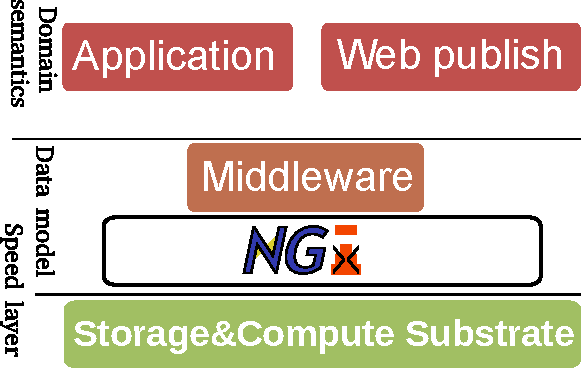
\includegraphics[width=0.75\columnwidth]{layers-ngi}
  \caption{Layers with NGI}
  \label{fig:ngilayers}
\end{figure}


\section{Next Generation Workflows}
\label{sec:ngWorkflows}

This section illustrates how workflows using NGI could be run and optimized by a smart runtime implementation of NGI.


\subsection{Climate/Weather in 2020+}

This workflow gives an idea how the climate and weather community could utilize emerging concepts in 2020+.
A generic overview of the workflows for climate and weather is given in \Cref{fig:climateWeather}.

Prediction of the weather in the near future (hours, known as nowcasting; days or weeks -- seasonal) is performed by executing workflows consisting of several processing steps. The execution of a workflow engine that orchestrates the individual execution steps is not explicitly included in the workflow description.

For weather prediction, these workflows are schedules on a regular basis, e.g., a prediction is performed every 4 hours. The prediction is based on observational data and outputs data products that are processed further and distributed to customers.

\subsubsection{Execution of a weather workflow}



\begin{figure}[b]
  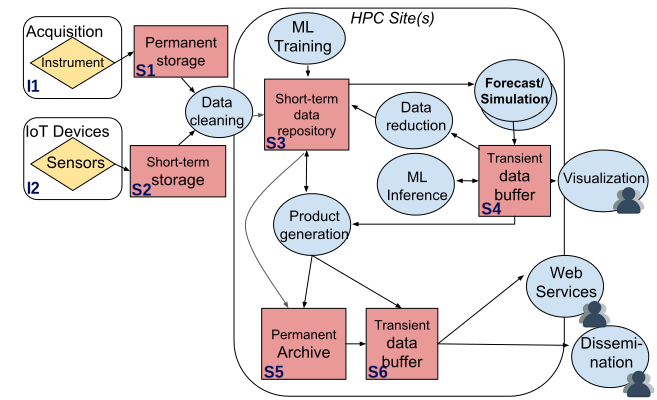
\includegraphics[width=\columnwidth]{climateweather-workflow}
  \caption{Future Climate and Weather Workflows}
  \label{fig:climateWeather}
\end{figure}


First, data sources providing up-to-date data (such as near-real-time satellite sources and weather stations, I1) are ingested into a local permanent repository (S1). These data may be supplemented by the increasing number of IoT and mobile sensor devices (I2) which data may be stored in a short-term storage (S2) with a limited life-time.
A weather service utilizing a HPC site ingests this data onto a local repository (S3). During this process, observational data is cleaned and reduced, e.g., by reducing resolution (subsampling).
An ensemble of forecasts (several parallel simulation applications) are started using a subset of the latest weather information -- typically each of the applications differs only in how the simulation is initialized.
They start with a warm up period using data from, e.g., 24 hours in the past. While a forecast runs it may use the data from I1/I2 to augment the simulated data with actual observations until the model time and the actual time matches and prediction of future weather starts.
While the ensemble of forecast runs, it computes various relevant output variables that may be stored in a transient data buffer (S4) and/or perform data transformation and analysis in-situ/in-transit. For example, a computed variables may be output, visualized and analyzed further by users even as the simulation continues. To identify patterns (events of interests for meteorologists), machine learning may be applied in the processing pipeline. Identified events may trigger further actions on the visualization, triggering additional data outputs, and controlling data reduction. To reduce the data volume for the ensemble, a data reduction selectively chooses data from the ensemble to preserve (on the repository S3, just before it is stored in the archive S5); this may be a typical run/minimum/maximum or runs that contain certain events as identified from the machine learning.
The generation of data products is either known beforehand, and calculated using a workflow during the ensemble run, or calculated post-mortem.
The former case is typical for weather applications. In the latter case, data products can be created offline from the stored output of the forecasts -- this allows users to request new or modified data products from the simulations via the web interface.
Machine learning can be applied in this workflow to identify relevant patterns in the data, supervised training involves the scientist selecting the phenomenon of interest presumably interactively using data visualization. The system should be able to quickly build a model and suggest other data with the similar phenomena to reduce the effort of the scientist to browse through all the data.

A selection of data products together are stored on a long-term (permanent) archive (S5).
Scientists over the world typically interact with web services to access data products on the long-term archive or to apply certain post-processing procedures to create new data products. This data is typically cached (S6) both at source before dissemination and by users in their workflow. When a new data product is requested it may actually trigger the recomputation of the data because it is cheaper than keeping all data products on a permanent storage.

Note that the box depicts “HPC-sites” that executes most parts of the workflow, however, not necessarily this must be a single data center. Scientists already work in a distributed fashion, downloading certain data products and performing subsequent data analysis locally, on other remote sites, data centers, or in the cloud. It is expected, thought, that the initial data production is kept on the site where the data is produced as the data volume is reduced significantly in this process.

\subsubsection{Execution of a climate workflow}

Generation of insight for a climate experiment differs from the weather case by several aspects: Firstly, the data (S2) from IOT devices (I2) is not used.
Secondly, in most cases scientists conduct new experiments, i.e., the result is a-prior unknown. Thus, a more exploratory and interactive use is expected.
For model intercomparison projects, once the variables and experiments to investigate are clear, a mass replication (execution) of the use case under different starting conditions takes place. These planned experiments come with less explorative nature, yet diagnosis of abnormal execution behavior may be investigated interactively.
Due to the vast amount of different experiments, the data management features of NGI are useful to simplify the data handling; for instance, by utilizing scientific metadata to specify the difference between different experiments differences between model output can be computed directly.


\subsection{Extreme Data Generation}

This section discusses a use case illustrating how the aforementioned concepts integrate into a smart system.
Consider the case in which a group of users conducts an experiment at large scale (a tightly coupled hero run on an HPC system) to gather new insight about small scale phenomenon.
This experiment generates raw data of a huge volume (e.g., several Petabytes on existing systems).
The user may know certain (diagnostic) post-processing that must be conducted on the data, but since the scientists work at the frontier of knowledge, it is usually unclear which features to look for and which data products to create.
Over a period of several month scientists will analyze a subset of data (e.g., two regions of 10 GiB each) potentially using machine learning to identify the further analysis steps that shall be conducted on the full dataset.
Once this is done, they register the analysis workflow and wait for all data products.

The user specifies the workflow defining the characteristics of the processing and the data and include that the final data product must be retained for 10 years.
The workflow also indicates that the data products are used in manual analysis and this may take several months.
Note that users do not deal with namespace issues but provide scientifically relevant metadata for the raw data and the data products.
At creation time of data products, these are semantically linked to the workflow and may be found when inspecting metadata for the created raw data.

\medskip

We envision the following support of the runtime for this use case:
The workflow description gives the scheduler various options; firstly, the final data product must be accessible for 10 years; it may decide that it is cost-efficient to store the data on a tape archive, a subset of the data region should be stored for in-depth analysis and likewise a low-resolution version of the should be created.
In another environment and depending on characteristics, the scheduler may have decided to not persist the huge data output but preserve a container for the application to allow recomputation -- but we will discuss the former case.

An I/O-enabled resource manager will dispatch the hero run exclusively once there is enough storage capacity available on the archive storage system such as tape and I/O bandwidth is available.
The system may schedule the post-processing, data reduction and subset creation, while  data transfer occurs in-transit on the client node or dedicated compute resources and picks a fast storage system for these products.
That means a data-driven streaming workflow is applied to minimize reading of data during the post-processing workflow.
The raw output is meanwhile directly stored on tape for archival purpose (e.g., as it must be kept for several years due to policies of the funding agency).
The sample data is a replicate of a subset of the raw data's domain and stored for inspection on a storage system supporting good random I/O workloads.
If a user inspects the metadata, one can see that fragments with a subset of data are stored on fast storage and the other parts on slow archival storage.
Once the user registers the final workflow, i.e., requests data processing on the full dataset, the system has to process the vast amount of data on tape.

Depending on the exact workflow, there are opportunities for the system:
Thanks to liquid computing, parts of the workflow can be executed directly on tape drives and the network thinning out the amount of data that needs to be transferred while reading.
Alternatively, we may retrieve the data from archive storage and create a copy on a faster storage system but -- since relevant parts of the workflow access pattern are known -- can reorganize the replicas of the fragment while data is fetched and, thus, optimize I/O for the subsequent accesses of the workflow.


\paragraph{In-Situ Analysis}

A user should be able any time to inspect and analyze data that is currently produced without changing the application code or even knowing a priori that this is an intent.
Let us extend the previous case of the hero run; now the user may decide to visually analyze a subset of data and a low-resolution output of the data while the data is generated.
We assume a node or visualization cluster has been allocated for this purpose.
An NGI enabled visualization tool would be able to query the metadata and search for the experiment currently conducted.
Then the region of interest is selected by the user.
In the best case, some derived data products could be reused but it is expected that the tool submits new tasks (code snippets for liquid computing) to the runtime to perform data analysis and reduction.
The system will create additional I/O streams and run the analysis codes in streaming mode as much as possible while it feeds the output to the application.
This would allow us to perform filter operations on the process creating the raw data.
If the volume of the produced data is too high, a workflow can be registered to create data products on the storage with good random I/O characteristics.
The visualization is then constantly updated according to the NGI semantics.

\subsection{Capacity Data Lifecycle Workflow}
The available storage solutions have changed over the years. One solution may work for a class of use cases, but not another class. The resulting environment is a heterogeneous hierchy of storage tiers. The tiers of data storage have varying levels of performance and different economic models. The trade-offs of these characteristics drives use cases. The need for a middleware translation layer is needed with various backend storage solutions whether Commercial off the shelf (COTS) solutions supplied or open source software (OSS) is crucial in an HPC ecosystem. 

Various data retention boundaries may not align with an HPC storage system’s lifetime. Due to constantly changing use cases and generational technology shifts a user may not be aware of proper use of a storage system. For example, a user may store a data set in HPSS, which is commonly use for a long term archival solution. This use then frequently recalls data from this solution. A more optimized use case would be to use Campaign Storage for warm active data sets. In some cases, workflow may not be known until a project progresses. 

Another unknown is future capabilities of a storage system. This also introduces significant effort in eduction, workflow optimization, and data stewardship. This can cause extra effort of system administrators and users alike. This future solution will address these challenges by giving a user more flexibility via workflow improvements. A generic overview of this workflow is given in \Cref{fig:dataLifecycle}

\begin{figure}[b]
  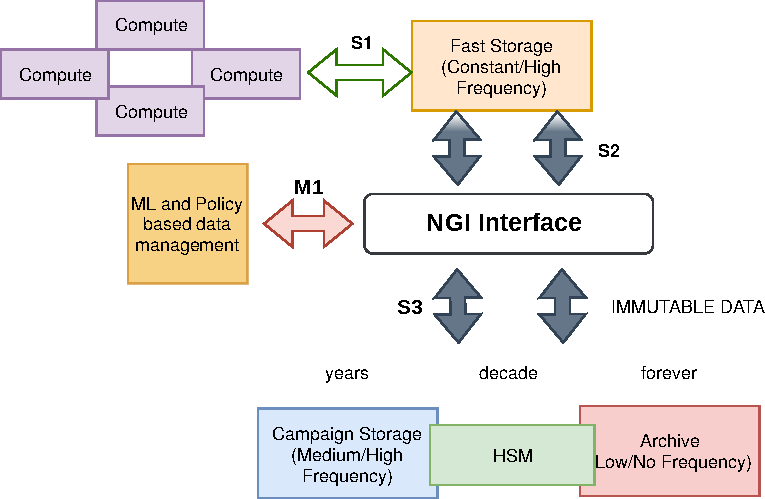
\includegraphics[width=0.75\columnwidth]{datalifecycle-workflow}
  \caption{Future Data Lifecycle Workflows}
  \label{fig:dataLifecycle}
\end{figure}

\subsubsection{Execution of the data lifecycle workflow}
First data sources are read and written from an HPC supercomputer. (S1) shows I/O between a compute and primay data store, that may be POSIX or another data store. This storage has high performance in bandwidth, latency and I/O operations. This data will be copied off this location via a data movement tool. (S2) is movement between the fast storage tier using Data Movers or File Transfer Agents (FTA). This FTA then on-the-fly tranlates from the native interface of one data store to the NGSI interface. This is depicted in (S2) and (S3). An additional layer of translation will occur at (S4), which translates the data to various storage backends. These backends are fully pluggable and customizable solutions. (M1) is Data Management and Machine Learning mechanisms or user defined migration policies and rules. (M1) works with the data movers to migrate data back and forth without manual user intervention. A user is able to read, write and delete immutable data and then allow for various data retention policies.


\paragraph{In-Situ Analysis}
The user will define data policies and the system administrator will devise ML techniques using empirical data models for optimized management and placement. The result is to use each storage tier in the intended use case with minimal effort of user. For example, a large dataset of hundreds of TiBs was put on a spinning disk archive (Campaign Storage), but only 10 GiB was accessed. A potential operation would be that through data policies migrate some, or most of it to a tape based system.

\section{Community Strategy}
\label{sec:community}

We are in the process to establish the NGI Forum that curates the development of the APIs.
The process will share the idea with the successful MPI Forum.
The approach is sketched in \Cref{fig:standardization};
members are experts from domain science, industry and data centers and form the bodies.
The activity is lead by the elected steering board.
Topic-specific workgroups and committees develop the standard (data model and APIs) driven by relevant use-cases encompassing the span from workflows to code snippets.
Ultimately, we will support the creation of a reference implementation based on state-of-the-art technology that demonstrates the approach on the use-cases.
We are aware that this endeavor is challenging; therefore, we won't expect that NGI 1.0 will include all features in the final version.
%We will settle on the set of features that the consortium identifies
%Similar to the way MPI 1.0 has grown, .

We expect that vendors and researchers will embrace the open ecosystem similarly to MPI and explore and contribute to the forum and its development.

\begin{figure}[b]
  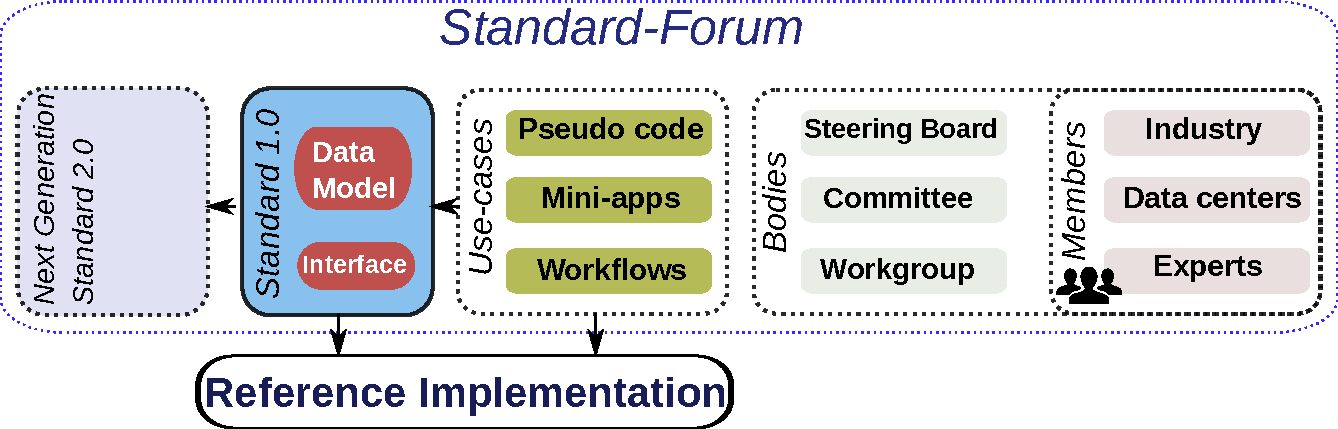
\includegraphics[width=\columnwidth]{standardization}
  \caption{Organization of the NGI Forum}
  \label{fig:standardization}
\end{figure}

\section{Conclusions}
\label{sec:conclusions}


Cloud definition of desired state and contracts.

Indeed many research prototypes address subproblems
* But not all aspects together
* Competing approaches; the standardization we describe here does not compete!

In this paper, we purposely do not mention too many of the ongoing RD\&E in storage and compute.




To wrap up, NGI provides a high-level view on data and processing on heterogeneous platforms while shielding the user from execution details.

Open ...


\includegraphics[width=2cm]{ngi-logo}

\noindent\url{https://ngi.vi4io.org}


\end{document}
